% author cany
\documentclass{beamer}

\usepackage{graphicx}
\usepackage{amsmath}
\usepackage{biblatex}
\usepackage{hyperref}
\usepackage{listings}
\usepackage{caption}
\usepackage{ amssymb }
\usepackage[utf8]{inputenc}
\usepackage{refcount}
\usepackage{tikz}
\usepackage{amssymb}
\usepackage{color, colortbl}
\usepackage{booktabs,array}  
\usepackage{caption}
\usepackage{bm}

\mode<presentation>
{
	\usetheme{Madrid}
	\setbeamercovered{transparent}
	\setbeamertemplate{caption}[numbered]
}
\beamertemplatenavigationsymbolsempty

\newcommand\pro{\item[$+$]}
\newcommand\con{\item[$-$]}

\title[Seminar Visual Computing] {MA-INF 2221 - Seminar Visual Computing}
\subtitle {DeepLab: Semantic Image Segmentation with Deep Convolutional Nets, Atrous Convolution, and Fully Connected CRFs } 
\author[Can Yuce]{Can Yuce\inst{1} \\
\texttt{yuce@uni-bonn.de}}
\institute[University of Bonn] 
{
	\inst{1}
	Department of Informatics\\
	University of Bonn
}
\date{\today}
\logo{\includegraphics[height=1.2cm]{uni-bonn.png}}

\begin{document}

\begin{frame}
	\titlepage
\end{frame}

\section{Outline}

\begin{frame}{Outline}
  \tableofcontents
\end{frame}

\section{Problem Statement and Motivation}

\begin{frame}{Semantic Image Segmentation}
\structure{Semantic segmentation is the task of}
\begin{itemize}
	\item recognizing/delineating objects,
	\item and classifying each pixel in an image.
\end{itemize}
\begin{figure}
	\centering
	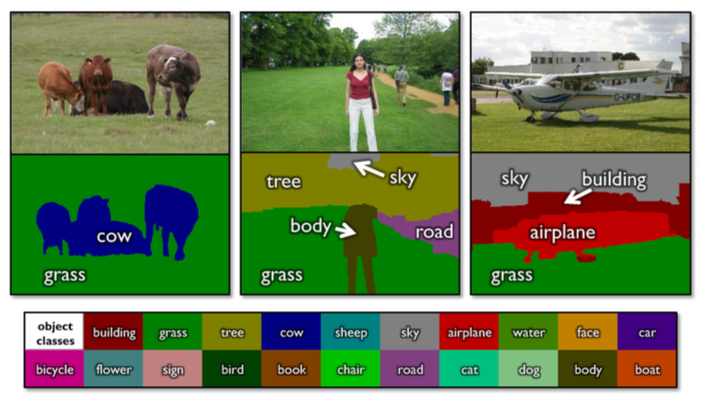
\includegraphics[width=0.5\textwidth]{figure/ss2.png}
	\captionsetup{justification=centering}
	\caption{TextonBoost applied to the MSRC 21 Class Database.\\Example semantic segmentation results\footnote{Shotton, Jamie, et al. "Textonboost for image understanding: Multi-class \\object recognition and segmentation by jointly modeling texture, layout, and context."}.\label{label1}}
\end{figure}
\end{frame}

\begin{frame}{Why is Semantic Segmentation Important?}
\structure{Road scene understanding}\\
\vspace{0.2cm}
\begin{itemize}
	\item
	Useful for autonomous navigation of cars and drones.
\end{itemize}
\begin{figure}
	\centering
	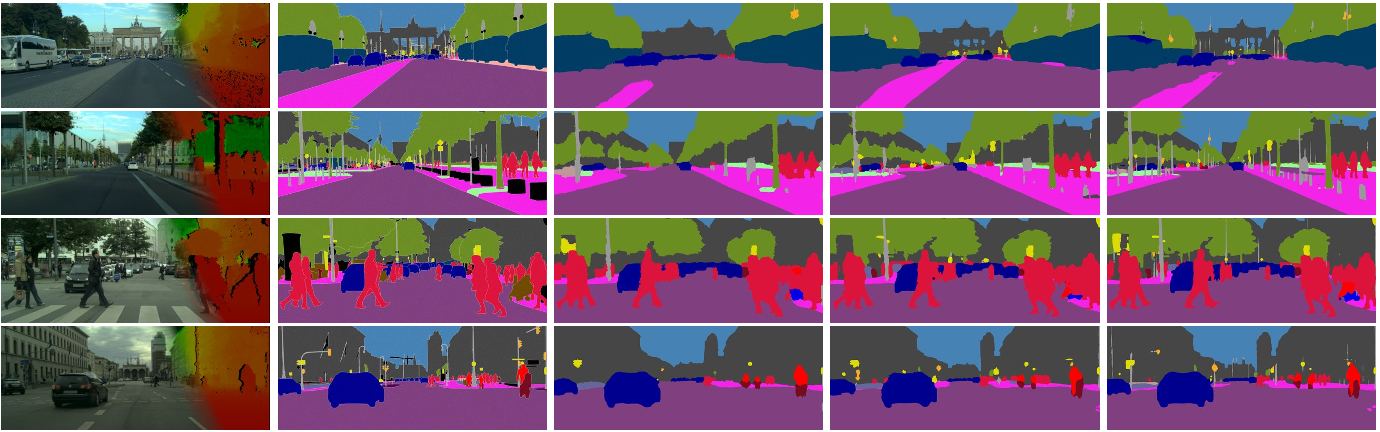
\includegraphics[width=0.8\textwidth]{figure/ss3.png}
	\captionsetup{justification=centering}
	\caption{The Cityscapes Dataset for Semantic Urban Scene Understanding\footnote{See more at \url{https://www.cityscapes-dataset.com.}}.}	
\end{figure}
\end{frame}

\begin{frame}{Why is Semantic Segmentation Important?}
\structure{Medical purposes}\\
\vspace{0.2cm}
\begin{itemize}
	\item
Segmenting tumours, organs, dental cavities etc.
\end{itemize}
\begin{figure}
	\centering
	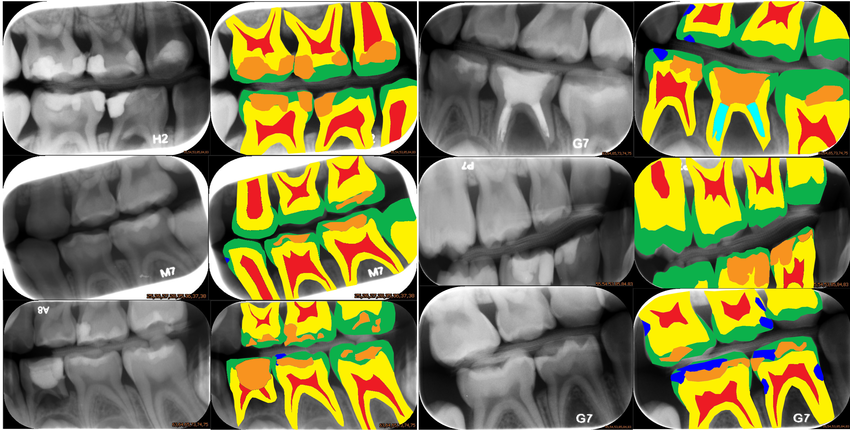
\includegraphics[width=0.7\textwidth]{figure/ss4.png}
	\captionsetup{justification=centering}
	\caption{Segmentation of dental cavities\footnote{Wang, Ching-Wei, et al. "A benchmark for comparison of dental \\ radiography analysis algorithms."}.}	
\end{figure}
\end{frame}

\begin{frame}{Why is Semantic Segmentation Important?}
\structure{Robot Vision}\\
\vspace{0.2cm}
\begin{itemize}
	\item
	To automatically segment objects from its background is important for active agents to interact(i.e. grasping, manipulation) effectively in the real world.
\end{itemize}
\begin{figure}
	\centering
	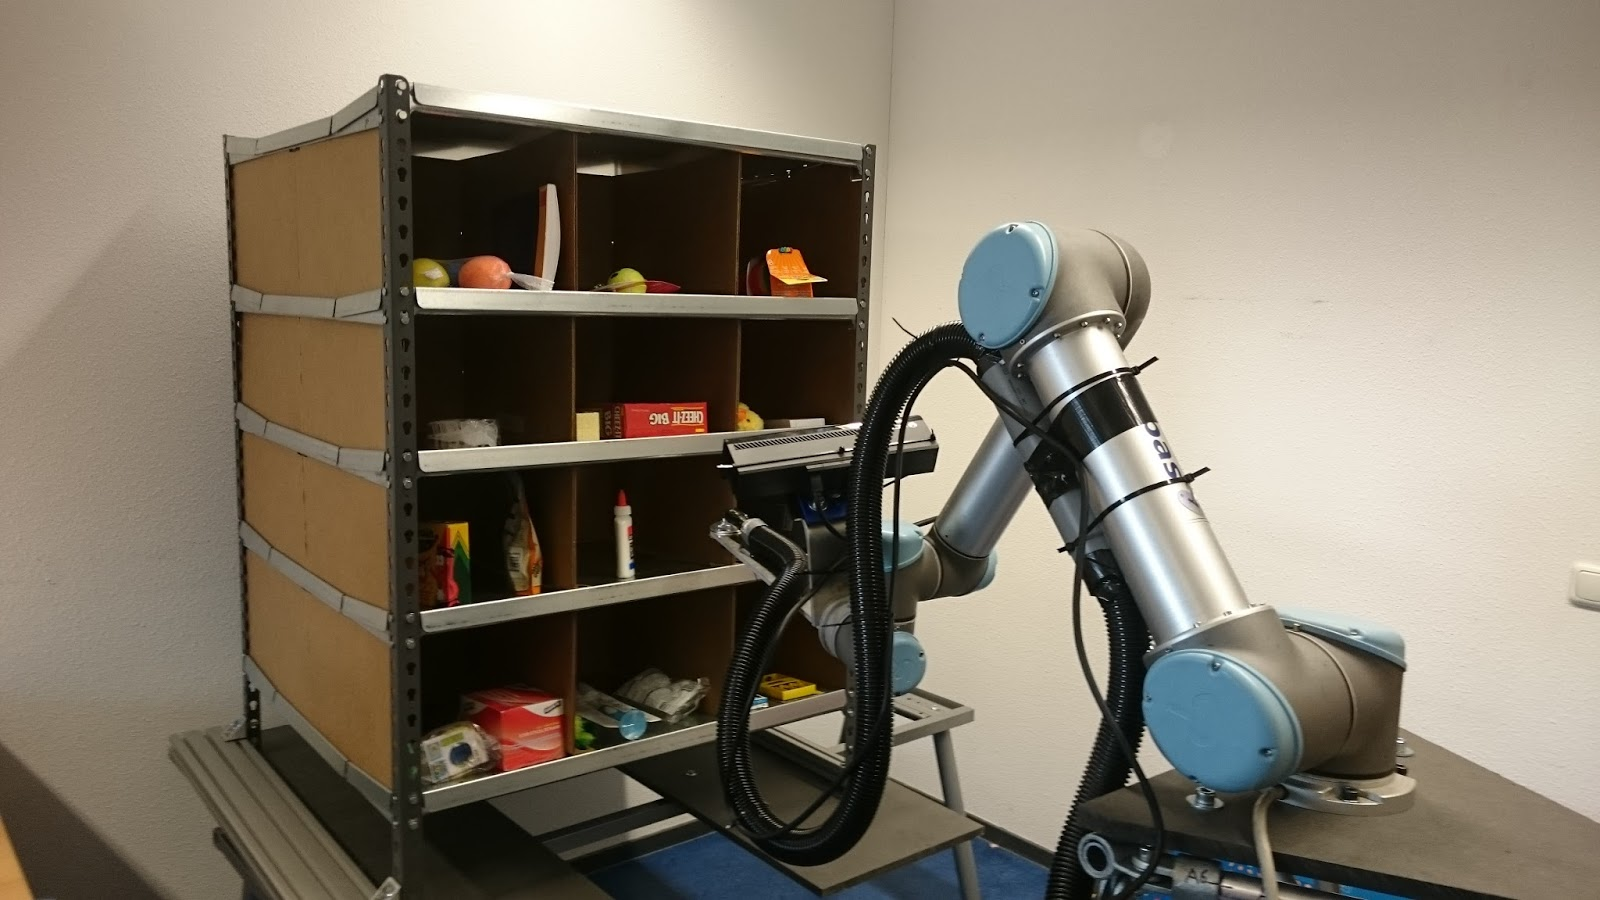
\includegraphics[width=0.5\textwidth]{figure/ss5.jpg}
	\captionsetup{justification=centering}
	\caption{A Vacuum Grapper tries to grasp objects from the shelf \footnote{\url{http://appliedrobotics.blogspot.de/2015\_08\_01\_archive.html}}.}	
\end{figure}

\end{frame}
\section{Connections with Other Work}
\begin{frame}{Semantic Segmentation Before Deep Learning}
\begin{figure}
	\centering
	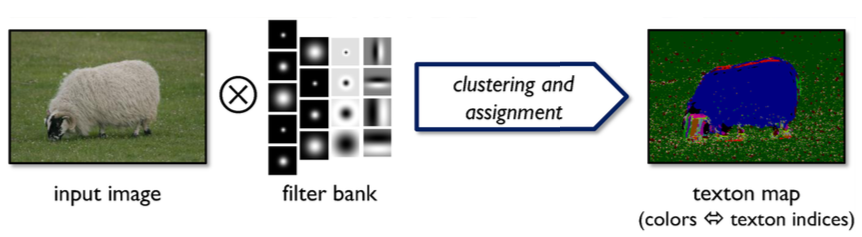
\includegraphics[width=0.5\textwidth]{figure/ss7.png}
	\captionsetup{justification=centering}
	\caption{The process of image textonization\footnotemark[\getrefnumber{label1}].}	
\end{figure}
	Most of the successful semantic segmentation systems used:
\begin{itemize}
	\item {\color{blue} Hand-crafted} features,
	\item<2-> Operations on {\color{blue}pixels} or {\color{blue}superpixels},
	\item<3-> Flat classifiers, such as {\color{blue} Boosting/Ensemble} methods,
	\item<4-> Models incorporating {\color{blue}local evidence} with interactions between {\color{blue}label assignments}.
	\item<5-> {\color{blue}Hierarchical classifiers} incorporating richer information from\\
	 context.
\end{itemize}
\end{frame}

\begin{frame}{Flat Classifiers}
\begin{figure}
	\centering
	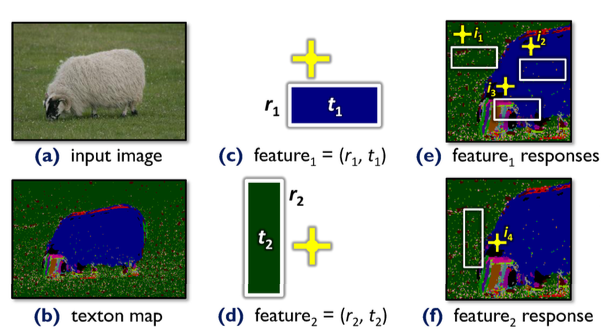
\includegraphics[width=0.5\textwidth]{figure/ss12.png}
	\captionsetup{justification=centering}
	\caption{Each weak learner is a decision stump based on the feature response\footnote{Shotton, Jamie, et al. "Textonboost for image understanding: Multi-class\\ object recognition and segmentation by jointly modeling texture, layout, and context."}.}	
\end{figure}
Boosting/Ensemble Methods, 
\begin{itemize}
	\item Random Forests, 
	\item Support Vector Machines etc.
\end{itemize}
\end{frame}	

\begin{frame}{CRF/MRF based Models}
 \begin{itemize}
	 \item {\color{blue}Conditional/Markov Random Fields} (CRF/MRF)are broadly used in semantic segmentation tasks.
	 \item {\color{blue}Unary classifiers} on single pixel/superpixels,
	 \item {\color{blue}Smoothness} terms that maximize label agreement between similar pixels.
\end{itemize}
\vspace{-0.4cm}
\begin{figure}
	\centering
	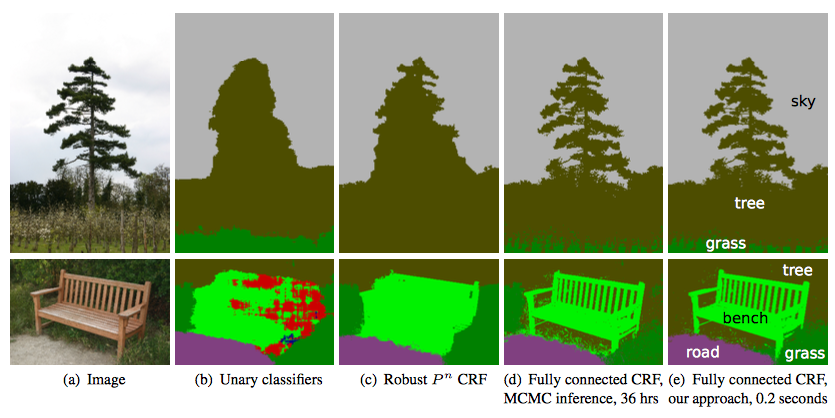
\includegraphics[width=0.64\textwidth]{figure/ss13.png}
	\captionsetup{justification=centering}
	\caption{Pixel-level classification with a fully connected CRF.\footnote{Philipp Krähenbühl, Vladlen Koltun. "Efficient Inference in Fully\\Connected CRFs with Gaussian Edge Potentials."}.}	
\end{figure}
\end{frame}

\begin{frame}{Hierarchical Models}
These methods benefit from allowing context to be incorporated at multiple levels of quantisation\footnote{Russell, Chris, et al. "Associative hierarchical crfs for object class image segmentation."}:
\begin{itemize}
	 \item The lowest layer of the image represents the pixel layer,
	 \item The middle layer potentials defined over super-pixels or segments
	 \item The third layer represents our hierarchical terms.
\end{itemize}
\begin{figure}
	\centering
	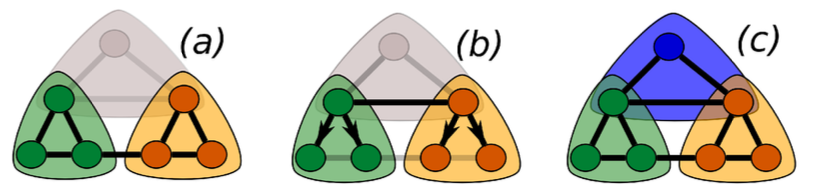
\includegraphics[width=0.64\textwidth]{figure/ss14.png}
	\captionsetup{justification=centering}
	\caption{Pixel-level classification with a fully connected CRF.}	
\end{figure}
\end{frame}

\begin{frame}{Deep Learning and Semantic Segmentation}
\begin{figure}
	\centering
	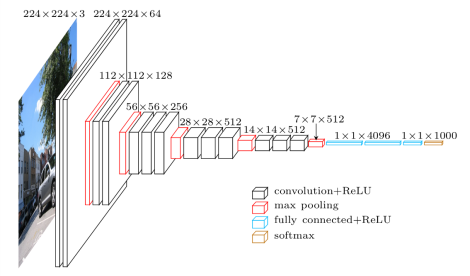
\includegraphics[width=0.5\textwidth]{figure/ss6.png}
	\captionsetup{justification=centering}
	\caption{VGG-16 network layer by layer\footnote{Simonyan, Karen, et al. "Very deep convolutional networks for large\\scale image recognition."}.}	
\end{figure}
\vspace{-0.6cm}
Deep Convolutional Neural Networks ({\color{blue}DCNN}) in classification:
\begin{itemize}
	\item {\color{blue}Input:} The whole image,
	\item {\color{blue}Output:} Probability of each class in image(a car, person, dog etc.)
	\item<2-> Not directly applicable to the Semantic Segmentation problem.
\end{itemize}
\end{frame}

\begin{frame}{DCNN + Region Proposals }
\begin{figure}
	\centering
	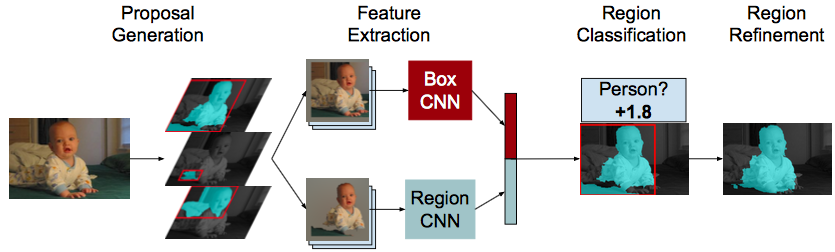
\includegraphics[width=0.75\textwidth]{figure/ss15.png}
	\captionsetup{justification=centering}
	\caption{Simultaneous Detection and Segmentation Pipeline.\footnote{Hariharan, Bharath, et al. "Simultaneous detection and segmentation, 2014."}.}	
\end{figure}
\vspace{-0.3cm}
\begin{enumerate}
	\item Employing a cascade of bottom-up image segmentation proposals/features,
\begin{itemize}
	\con Fail to recover from any of its errors.
\end{itemize}
	\item <2->DCNN-based regional classification,
	\item <3->Refining proposals.
\end{enumerate}
\end{frame}

\begin{frame}{DCNN Features + Segmentation Proposal}

\begin{figure}
	\centering
	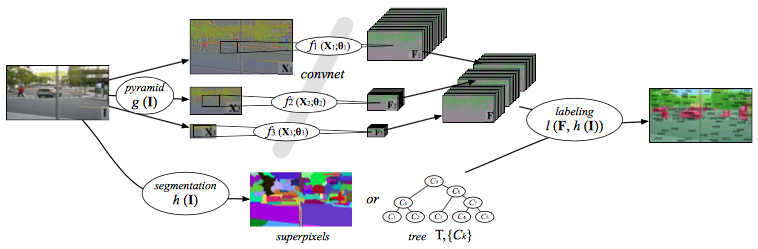
\includegraphics[width=0.85\textwidth]{figure/ss16.png}
	\captionsetup{justification=centering}
	\caption{Scene labeling system\footnote{Farabet, Clement, et al. "Learning hierarchical features for scene labeling (2013)."}.}	
\end{figure}
\vspace{-0.5cm}
\begin{enumerate}
	\item Employ DCNNs at multiple image resolutions,
	\item<2-> Construct a segmentation tree to smooth the prediction results,
	\item<3-> Segmentation algorithms are decoupled from the DCNN classifier’s results.
	\begin{itemize}
		\con Risking commitment to premature decisions.
	\end{itemize}
\end{enumerate}
\end{frame}

\begin{frame}{Dense Prediction}
\begin{itemize}
	\item {\color{blue}Arbitrary input size: } Take input of arbitrary size and produce {\color{green}correspondingly-sized} output efficiently.
	\item<2->{Transforming all the {\color{red}fully connected layers} to {\color{green}convolutional layers} enables a classification net to output a heatmap\footnote{Long, Jonathan, et al. "Fully convolutional networks for semantic segmentation."}).}	
	\item<3-> Transfer learning using pretrained DCNN(i.e. VggNet, Resnet).
	\end{itemize}
	\vspace{-0.1cm}
	\begin{figure}
		\centering
		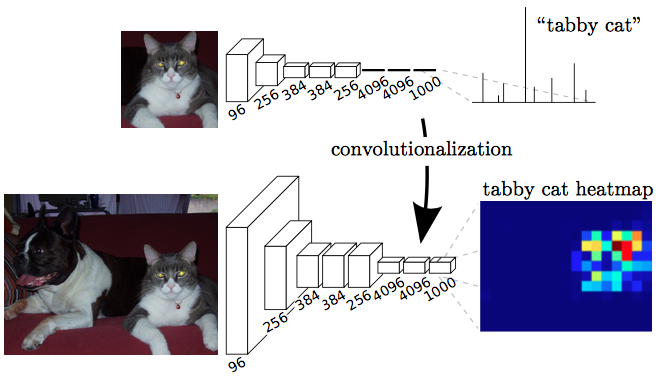
\includegraphics[width=0.5\textwidth]{figure/ss40.png}
		\captionsetup{justification=centering}
		\caption{Transforming all the fully connected layers to \\convolutional layers.}	
	\end{figure}
\end{frame}

\section{Challenges}

\begin{frame}{Challenges}
	\only<1>{Challenges in the application of DCNNs on semantic image segmentation:}
\begin{enumerate}
	\only<1->{\item {\color{blue}Reduced feature resolution}: Caused by the repeated combination of max-pooling(downsampling) performed at consecutive layers of DCNNs originally designed for image classification.}
	\only<1>
	{ \begin{figure}
		\centering
		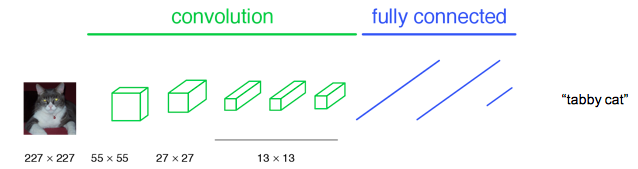
\includegraphics[width=0.65\textwidth]{figure/ss8.png}
		\captionsetup{justification=centering}
		\caption{A classification network\footnote{Long, Jonathan, et al. "Fully convolutional networks for semantic segmentation."}.}	
\end{figure} }

\only<2-> {
	\begin{itemize}
		\item<2-> {\color{blue}Solution \#1}: Convert coarse outputs to dense pixels using interpolation. i.e. simple {\color{magenta}bilinear interpolation}.
	    \begin{itemize}
			\pro Fast.
			\con Not efficient as the operation is not learnable.
		\end{itemize}
		\item<3-> {\color{blue}Solution \#2}: Convolution with fractional strides.  i.e. {\color{magenta}deconvolution}\footnote{Long, Jonathan, et al. "Fully convolutional networks for semantic segmentation."}.
		    \begin{itemize}
			\pro Slow.
			\con Can be learned, thus efficient(fast).
		\end{itemize}
		\item<4-> {\color{blue}Solution \#3}: DCNN without max-pooling layers. 
		\begin{itemize}
			\pro Can be learned.
			\con Discriminative ability owes much of their power to max-pooing layers.
		\end{itemize}
	\end{itemize}
}
\end{enumerate}
\end{frame}

\begin{frame}{Challenges}
\begin{enumerate}
	\setcounter{enumi}{1}
	\item {\color{blue}Existence of objects at multiple scales}
\begin{itemize}
	\item{ShareNet: Resizes the input image to several scales and passes each through a shared deep network\footnote{Chen, Liang-Chieh, et al. "Attention to scale: Scale-aware semantic image segmentation."}.}	
	\item<2->{Define scale-invariant mean squared error\footnote{Eigen, David, et al. "Depth map prediction from a single image using a\\ multi-scale deep network."}:}
	\begin{align*}
	D(y,y^{*})	&= \frac{1}{2n}\sum_{=1}^{n}\left( \log{y_i}-\log{y_{i}^{*}}+a(y,y^{*})\right)^2 \\
	\text{where, } \alpha(y,y^{*}) &= \frac{1}{n}\sum_{i}\left( \log{y_{i}^{*}}-\log{y_i}\right)
	\end{align*}
\end{itemize}
	\end{enumerate}
\end{frame}

\begin{frame}{Challenges}
\begin{enumerate}
	\setcounter{enumi}{1}
	\item {\color{blue}Existence of objects at multiple scales}
	\begin{itemize}
		\item{Spatial pyramid pooling\footnote{He, Kaiming, et al. "Spatial pyramid pooling in deep convolutional networks for visual recognition (2014)."}: Generates a fixed-length representation regardless of image size/scale}			
	\end{itemize}
\end{enumerate}
\begin{figure}
	\centering
	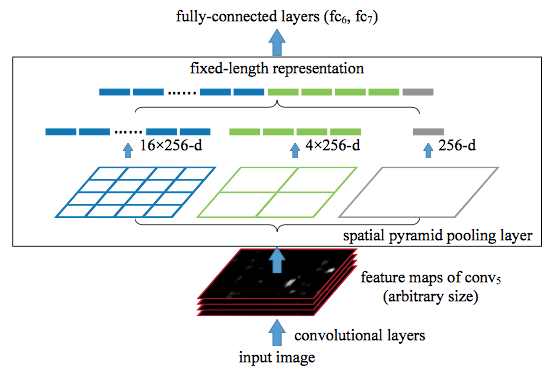
\includegraphics[width=0.5\textwidth]{figure/ss17.png}
	\captionsetup{justification=centering}
	\caption{Network structure with a spatial pyramid pooling layer.}	
\end{figure}
\end{frame}


\begin{frame}{Challenges}
\begin{enumerate}
	\setcounter{enumi}{2}
	\item {\color{blue}DCNN has limited {\color{blue}spatial capacity}}:  Invariance to spatial transformations limits the spatial accuracy of a DCNN.

	\begin{itemize}
		\item SkipNet: Features from intermediate layers are fused to produce the final output\footnote{Long, Jonathan, et al. "Fully convolutional networks for semantic segmentation."\label{note1}}.
	\end{itemize}	
	\begin{columns}
		\begin{column}{0.5\textwidth}
			\begin{figure}
				\centering
				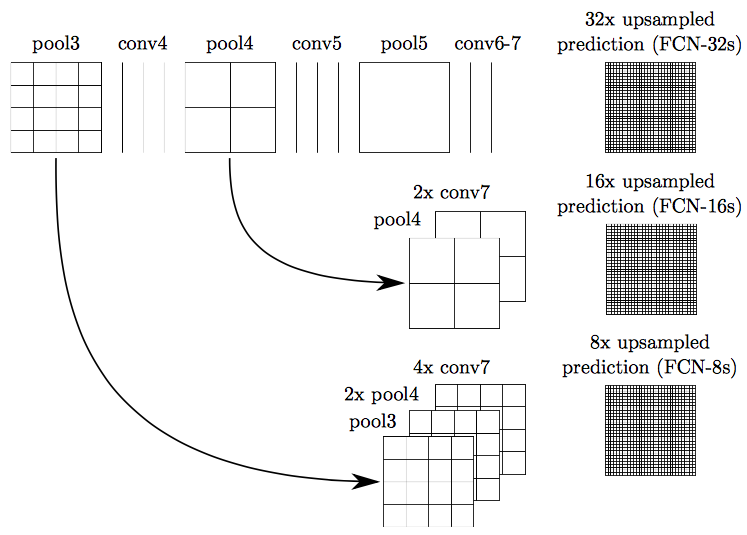
\includegraphics[width=5cm,height=3.5cm]{figure/ss10.png}
				\captionsetup{justification=centering}
				\caption{SkipNet Architecture.}	
			\end{figure}
		\end{column}
		\begin{column}{0.5\textwidth}  
			\begin{center}
			\begin{figure}
				\centering
				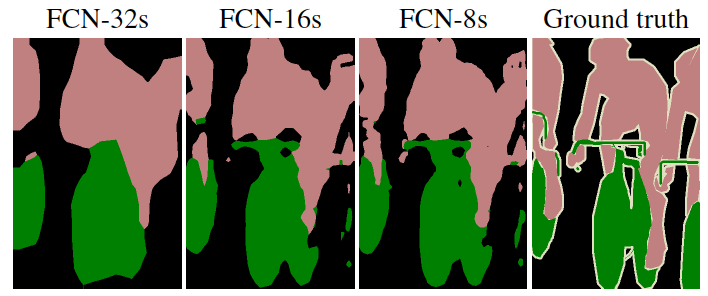
\includegraphics[width=5cm,height=2.5cm]{figure/ss27.png}
				\captionsetup{justification=centering}
				\caption{Refining fully convolutional nets by fusing information from layers with different strides\footnotemark[\getrefnumber{note1}].}
			\end{figure}
			\end{center}
		\end{column}
	\end{columns}
\end{enumerate}
\end{frame}

\begin{frame}{Challenges}
\begin{enumerate}
	\setcounter{enumi}{2}
	\item {\color{blue}DCNN has limited {\color{blue}spatial capacity}}:  Invariance to spatial transformations limits the spatial accuracy of a DCNN.
	\begin{itemize}
		\item Hypercolumns: Compute the outputs of all units above the locations at all layers of the CNN, stacked into one vector\footnote{Hariharan, Bharath, et al. "Hypercolumns for object segmentation."}.
	\end{itemize}	
	\begin{figure}
		\centering
		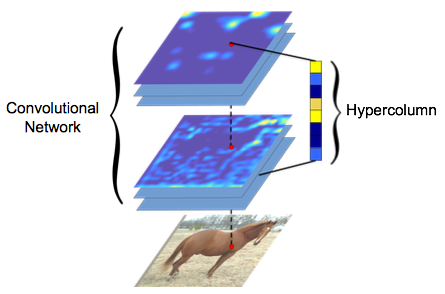
\includegraphics[width=0.45\textwidth]{figure/ss20.png}
		\captionsetup{justification=centering}
		\caption{Hypercolumns}	
	\end{figure}
\end{enumerate}
\end{frame}

\section{DeepLab: Key Technical Ideas}

\begin{frame}{Key Technical Ideas}
\begin{figure}
	\centering
	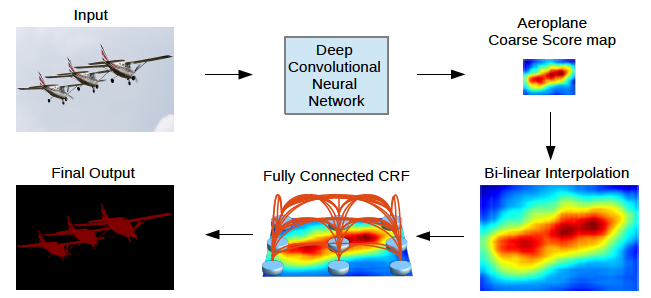
\includegraphics[width=0.6\textwidth]{figure/ss18.png}
	\captionsetup{justification=centering}
	\caption{Model Illustration.}	
\end{figure}
\vspace{-0.4cm}
	\begin{itemize}
	\item VGG-16/Resnet-101 trained on ImageNet dataset is employed in a {\color{blue}fully convolutional} fashion,
	\item<2-> Atrous convolution to reduce the degree of signal downsampling (from $32\times$ down to $8\times$).
	\item<3-> {\color{blue}Bilinear interpolation} stage to enlarge the feature maps.
	\item<4-> A fully connected CRF applied to refine the segmentation result.
\end{itemize}	
\end{frame}

\section{DeepLab: Main Contributions}
\begin{frame}{Atrous Convolution}
\vspace{-0.15cm}
\begin{figure}
	\centering
	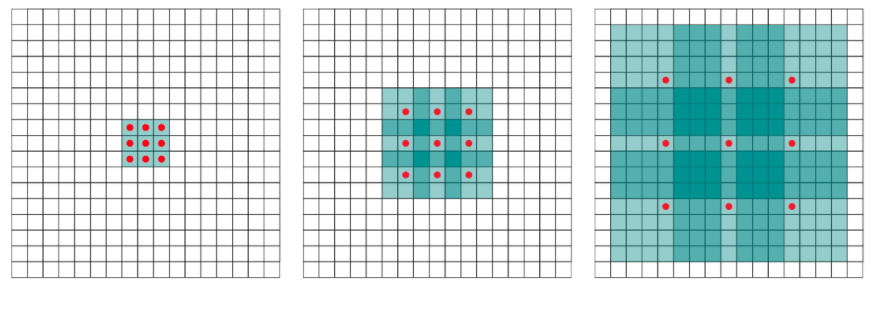
\includegraphics[width=0.6\textwidth]{figure/ss19.png}
	\captionsetup{justification=centering}
	\vspace{-0.25cm}
	\caption{Atrous filtering\footnote{Yu, F. (2015) Multi-scale context aggregation by dilated convolutions. }.}	
\end{figure}
\begin{itemize}
	\vspace{-0.45cm}
	\item Allows to compute the responses of any layer at any desirable resolution.
	\item<2-> Inspired from the {\color{blue}dilating filters} used in stationary wavelet transform(\textit{algorithme \'a trous\footnote{Holschneider, Matthias, et al. "A real-time algorithm for signal analysis with the help of the wavelet transform. (1989)"}}).
	\item<3-> The output $y[i]$ of atrous convolution where {\color{blue}r} is the \textit{rate} parameter:
	\vspace{-0.15cm} 
	\begin{align*}
		y\left[i\right] =\sum_{k=1}^{K}x[i+r\cdot k]w[k] 
	\end{align*}		
\end{itemize}	
\end{frame}

\begin{frame}{Atrous Convolution}
\begin{figure}
	\centering
	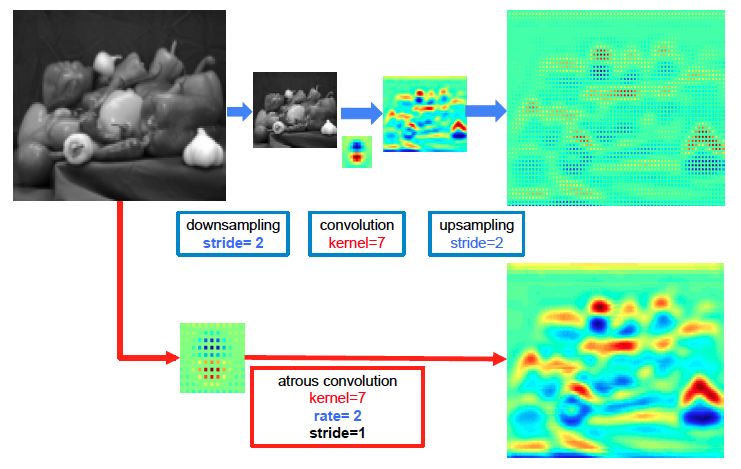
\includegraphics[width=0.5\textwidth]{figure/ss44.png}
	\captionsetup{justification=centering}
	\caption{Atrous filtering in 2D}	
\end{figure}
\vspace{-0.4cm}
\begin{itemize}
	\item Trick: Allows to preserve/enlarge image resolution and enlarge FOV at once.
	\item<2-> Subsampling leads to sparse feature extraction. Therefore, upsampled features are sparse as well.
	\item<3-> Number of filter parameters remains the same.
	\item<4-> Learnable and memory/time efficient.
\end{itemize}	
\end{frame}

\begin{frame}{Atrous Convolution}
\begin{table}[]
	\centering
	\caption{$\text{VGG}_{16}$: 224x224x3 input image; 1x1000 output labels.}
	\vspace{-0.3cm}
	\label{my-label}
	\resizebox{\textwidth}{!}{%
		\begin{tabular}{c|c|c|c|c|c|c|c|c|c|c|c|c}
			\hline	
			& 1                 & 2            & 3                 & 4            & 5                 & 6            & 7                 & 8            & 9                 & 10           & 11            & 12          \\
			\hline	
			layer & \textbf{2xconv} & \textbf{max} & \textbf{2xconv} & \textbf{max} & \textbf{3xconv} & \textbf{max} & \textbf{3xconv} & \textbf{max} & \textbf{3xconv} & \textbf{max} & \textbf{2xfc} & \textbf{fc} \\
			fs    & 3-1               & 2-2          & 3-1               & 2-2          & 3-1               & 2-2          & 3-1               & 2-2          & 3-1               & 2-2          & -             & -           \\
			\#cha & 64                & 64           & 128               & 128          & 256               & 256          & 512               & 512          & 512               & 512          & 1             & 1           \\
			act   & relu              & idn          & relu              & idn          & relu              & idn          & relu              & idn          & relu              & idn          & relu          & soft        \\
			size  & 224               & 112          & 112               & 56           & 56                & 28           & 28                & 14           & 14                & 7            & 4096          & 1000 \\
			\hline	
		\end{tabular}%
	}
\end{table}

\begin{itemize}
	\item The last two max-pooling layers are of $2\times2$ filters with {\color{blue}stride 1}. 
	\item Reduce the degree of signal downsampling (from $32\times$ down $8\times$).
	\item {\color{blue}Modify VGG-16 net:}
	\begin{itemize}
	\item $r=2$ atrous filters in layers:  {\color{blue}conv5\_1, conv5\_2 and conv5\_3}.
	\item $r=4$ atrous filter in the first fully-connected layer({\color{blue}fc6}).
	\item Bilinear filter($8\times$) in the last fully-connected layer({\color{blue}fc8}).
	\end{itemize}
	%\item From 32x down 1x is possible but expensive.
\end{itemize}	
\end{frame}

\begin{frame}{Atrous Convolution}
\begin{table}
	\setlength{\tabcolsep}{3pt}
	\begin{tabular}{ c c c | c }
		\hline
		\rule{0pt}{2.5ex}    
		Kernel & Rate & FOV  & \textbf{Params} \\
		\hline
		7x7 & 4 & 224 & 134.3M\\
		4x4 & 4 & 128 & 65.1M\\	
		4x4 & 8 & 224 & 65.1M\\
		3x3 & 12 & 224 & 20.5M\\	
		\hline					
\end{tabular}
\captionsetup{justification=centering}
\caption{Effect of kernel size on FOV.}	
\end{table}

\vspace{-0.4cm}
\begin{itemize}
	\item Direct adaptation of VGG-16 net using $7\times7$ kernel size and $r=4$.
	\item<2-> Improved model speed by reducing the kernel size to $4\times4$.
	\con<2-> Fails to capture local detail when \textit{rate} is increased.
\end{itemize}	
\end{frame}

\begin{frame}{Atrous Spatial Pyramid Pooling (ASPP)}
\begin{figure}
	\centering
	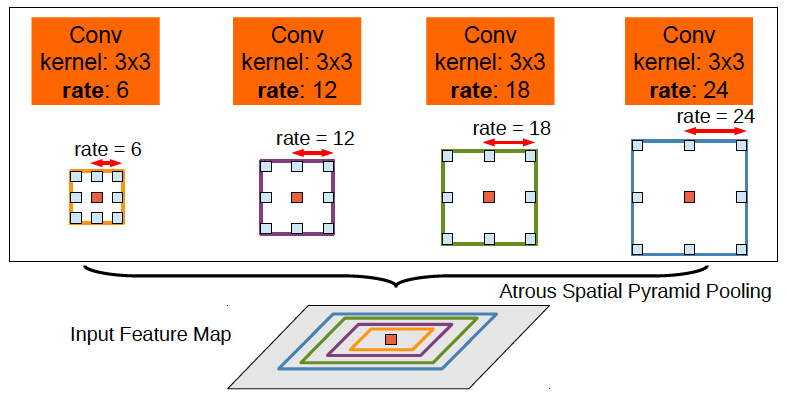
\includegraphics[width=0.7\textwidth]{figure/ss24.png}
	\captionsetup{justification=centering}
	\caption{Atrous Spatial Pyramid Pooling (ASPP).}	
\end{figure}
\vspace{-0.4cm}
\begin{itemize}
%	\item DCNNs already can represent multi-scale objects.
%	\item Multiscale processing significantly improves performance but expensive.
    \item The network should be able to handle objects at mutiple scale.
	\item ASPP extracts multi-scale features by employing multiple parallel filters with different rates on the same feature map.
\end{itemize}	
\end{frame}

\begin{frame}{Atrous Spatial Pyramid Pooling (ASPP)}
\vspace{-0.5cm}
\begin{figure}
	\centering
	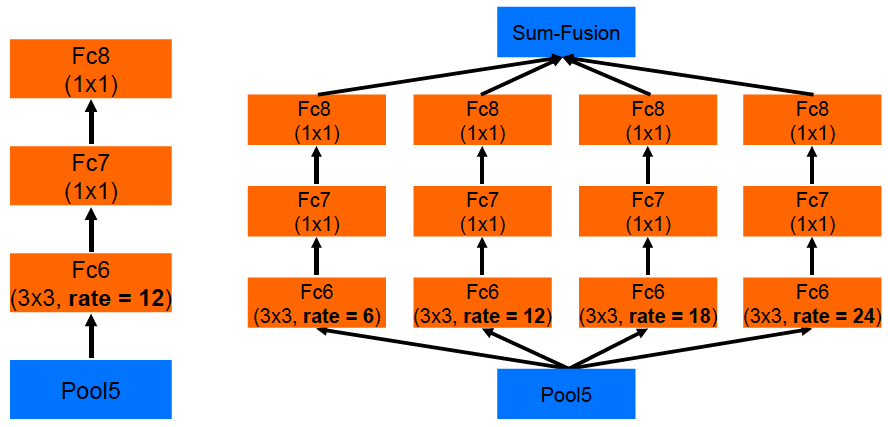
\includegraphics[width=0.7\textwidth]{figure/ss43.png}
	\captionsetup{justification=centering}
	\caption{Atrous Spatial Pyramid Pooling (ASPP).}	
\end{figure}
\vspace{-0.4cm}
\begin{itemize}
	\item Inspired from 
	{\color{blue} Spatial Pyramid Pooling}\footnote{He, Kaiming, et al. "Spatial pyramid pooling in deep convolutional networks for visual recognition (2014)."}.
	\item<2-> ASPP for VGG-16 employs several parallel fc6-fc7-fc8 branches.
	\item<2-> Four branches and smaller atrous rates  $r=\{6,12,18,24\}$.
\end{itemize}	
\end{frame}

\begin{frame}{Fully Connected CRF}
\begin{figure}
	\centering
	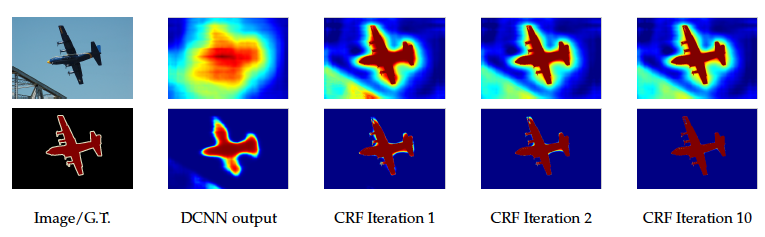
\includegraphics[width=0.7\textwidth]{figure/ss26.png}
	\captionsetup{justification=centering}
	\caption{Score map (input before softmax function) and belief map (output of softmax function) for Aeroplane.}
\end{figure}
\vspace{-0.4cm}
\begin{itemize}
	\item Large receptive fields can only yield smooth responses.
	\item CRF helps us to recover object boundaries at a level of detail.
	\item<2-> Short-range CRF is detrimental: results in excessive smoothing of object boundaries\footnote{Krähenbühl et al. "Efficient inference in fully connected crfs with \\Gaussian edge potentials."}.
	\item<2-> To overcome these problems, {\color{blue}fully connected CRF} is utilized.
\end{itemize}	
\end{frame}

\begin{frame}{Fully Connected CRF}
	\vspace{-0.4cm}
\begin{figure}
	\centering
	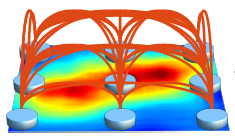
\includegraphics[width=0.3\textwidth]{figure/ss28.png}
	\captionsetup{justification=centering}
	\caption{Fully Connected CRF.}	
\end{figure}
\vspace{-0.4cm}
\begin{itemize}
	 \item Gibbs energy\footnote{Krähenbühl et al. "Efficient inference in fully connected crfs with \\ Gaussian edge potentials."} corresponding to FC-CRF is
	\begin{align*}
	E(x) =\sum_{i}\theta_i(x_i)+\sum_{ij}\theta_{ij}(x_i,x_j)
	\end{align*}
	where $x$ is the label assignment and $ij$ are pixel pairs. 
	\item<2-> Unary potentials are 
	\vspace{-0.4cm}
	\begin{align*}
	\theta_i(x_i)=-logP(x_i)
	\end{align*}
	where $P(x_i)$ is the label assignment probability at pixel $i$ computed \\by DCNN. 
\end{itemize}
\end{frame}

\begin{frame}{Fully Connected CRF}
\begin{itemize}
	\item MAP labeling by the unary classifiers alone is noisy and inconsistent. 
	\item<2-> Pairwise potentials are utilized:
	\begin{align*}	
	\theta_{ij}(x_i,x_j)=\mu(x_i,x_j)\left[ w_1exp\left(-\frac{\lVert \mathbf{p_i-p_j} \rVert^2}{2\sigma_\alpha^2}-\frac{\lVert  \mathbf{I_i-I_j} \rVert^2}{2\sigma_\beta^2} \right) \right. \\ 
	\left. + w_2exp\left(-\frac{\lVert \mathbf{p_i-p_j} \rVert^2}{2\sigma_\gamma^2}\right)   \right] 
	\end{align*}
	where $\mu(x_i,x_j)=1$ if $x_i \neq x_j$ and zero otherwise. 
	\item<3-> Gaussian potentials are calculated in different feature spaces.
\end{itemize}
\end{frame}

\begin{frame}{Fully Connected CRF}
\begin{itemize}
	\item<1-> Gaussian CRF potentials in the {\color{blue}fully connected CRF} model can capture long-range dependencies.
	\item<2-> Model is amenable to efficient fast {\color{blue}mean field inference}\footnote{Krähenbühl et al. "Efficient inference in fully connected crfs with gaussian edge potentials."}.
	\item<3-> Mean field methods perform {\color{blue}approximate probabilistic inference} by searching within a tractable subset of distributions\footnote{Nowozin, Sebastian, and Christoph H. Lampert. "Structured learning and prediction in computer vision."}.
	\item<4-> Key idea: if {\color{blue}kernel/pairwise cost function} is Gaussian, {\color{blue}message passing} can be performed via Gaussian filtering in feature space.
	\item<5-> Reduces the complexity of message passing from quadratic to {\color{blue} linear}. Inference requires  $<0.5$ secs on a CPU. {\color{red}Graph cut inference} in the fully connected models takes $>72$ hours.
\end{itemize}
\end{frame}

\section{DeepLab: Experimental Set-Up }
\begin{frame}{DeepLab: Experimental Set-Up }
\begin{itemize}
	\item VGG-16 and ResNet-101 trained on ImageNet\footnote{Krizhevsky, Alex et al. "Imagenet classification with deep convolutional neural networks."} dataset are employed.
	\item<2-> Evaluation is perfomed on {\color{blue}PASCAL VOC 2012}, {\color{blue}PASCAL-Context}, 	{\color{blue}PASCAL-Person-Part}, and {\color{blue}Cityscapes datasets}.  \onslide<2->
	\item<3-> 1000-way Imagenet classifier in the last layer is replaced with a classifier having the number of semantic classes.\onslide<3->
	\item<4-> DCNN and CRF training stages are decoupled.  
\end{itemize}
\end{frame}

\begin{frame}{DeepLab: Experimental Set-Up }
\begin{itemize}
	\item Loss function is the sum of cross-entropy terms for each pixel in the CNN output map. Cross-entropy error function is,
	\begin{align*}
	\mathcal{H}(\mathbf{o},\mathbf{t})=-\sum_{i=0}^{n}\log(o_i)\cdot t_i
	\end{align*}
	where, $o_i$ is the predicted probability distribution and $t_i$ is the true probability of class $i$. 
	\item<2-> CNN output map and GT labels are subsampled by 8 compared to the original image.
	\item<3-> Labels are mildly unbalanced\footnote{Long, Jonathan, et al. "Fully convolutional networks for semantic segmentation."} (about 3/4 are background). Hence, all labels are equally weighted when loss function is computed.
	\item<4-> Stochastic Gradient Descent method is utilized\footnote{Bottou, Léon. "Large-scale machine learning with stochastic gradient\\ descent." (2010)}. 
\end{itemize}
\end{frame}

\begin{frame}{DeepLab: Experimental Set-Up }
Main contributions implemented and tested:
\begin{itemize}
	\item {\color{blue}Atrous Filter}: Single branch, (kernel size $4\times4$, $r=4$).	
	\item {\color{blue}LargeFOV}: Single branch, (kernel size $3\times3$, $r=12$) atrous filter.
	\item {\color{blue}ASPP-S}: Four branches, $r= \{2, 4, 8, 12\}$.
	\item {\color{blue}ASPP/ASPP-L}: Four branches, $r = \{6, 12, 18, 24\}$.
	\item {\color{blue}CRF}: Fully Connected CRF.
\end{itemize}
Other methods:
\begin{itemize}
	\item {\color{blue}MSC}: multi-scale inputs are fed to the DCNN images at scale = $\{0.5, 0.75, 1\}$ with max-fusion.
	\item {\color{blue}COCO}: models pretrained on MS-COCO dataset.
	\item {\color{blue}Aug}: randomly scaled input images from 0.5 to 1.5.
	\item {\color{blue}ResNet-101\footnote{He, Kaiming, et al. "Deep residual learning for image recognition. (2016)"}}: deeper network trained on ImageNet dataset. 
\end{itemize}
\end{frame}

\begin{frame}{DeepLab: Experimental Set-Up }
	\vspace{-0.5cm}
\begin{figure}
	\centering
	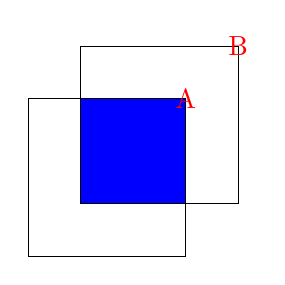
\begin{tikzpicture}
	
		\begin{scope}
		\clip (0,0) rectangle (2,2);
		\fill[blue] (-2/3,-2/3) rectangle (4/3,4/3);
		\end{scope}
		\draw (0,0) rectangle (2,2) node[red] {B};
		\draw (-2/3,-2/3) rectangle (4/3,4/3) node[red] {A};
	\end{tikzpicture}
	\caption{Intersection-over-union(IOU) } \label{fig:M1}
\end{figure}
\vspace{-0.5cm}
\begin{itemize}
	\item Evaluation metric is pixel intersection-over-union ({\color{blue}IOU}) averaged across the classes.
\begin{align*}
	\text{score} = 100\times\left[ \frac{\text{area of overlap}(A\cap B)}{\text{area of union}(A\cup B)}\right] 
\end{align*}
\end{itemize}

\end{frame}
\begin{frame}{Pascal VOC 2012: Dataset}
\begin{figure}
	\centering
	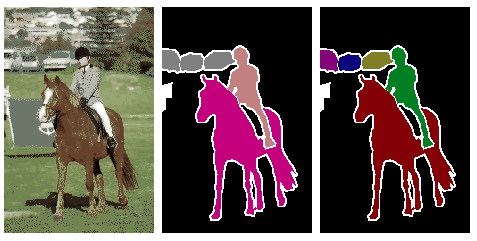
\includegraphics[width=0.50\textwidth]{figure/ss36.png}
	\captionsetup{justification=centering}
	\caption{Pascal VOC 2012 Dataset.}
	\label{fig:M5}
\end{figure}
\vspace{-0.5cm}
\begin{itemize}
	\item 20 foreground object classes and one background class\footnote{Everingham, M., et al. "The pascal visual object classes challenge 2012\\ (voc2012) results (2012)."}.
	\item {\color{blue}1,464} (\textit{train}), {\color{blue}10,582} (\textit{trainaug}),  {\color{blue}1,449} (\textit{val}), and  {\color{blue}1,456} (\textit{test}) pixel-level labeled images.
	\item Example of segmentation ground truth is shown in {\color{blue}Figure \ref{fig:M5}}.
\end{itemize}
\end{frame}

\begin{frame}{Pascal VOC 2012: Evaluation}
\begin{itemize}
	\item<1-> VGG-16 and ResNet-101 networks pre-trained on Imagenet are used.
	\item<2-> {\color{blue}Momentum} and {\color{blue}weight decay} are set to $0.9$ and $0.0005$ respectively.
	\item<3-> 10 mean field iterations.
	\item<4-> The number of filters in fc6/fc7 layers reduced from 4096 to 1024.

\begin{itemize}
	\pro Enables 3.36 times faster training speed.
\end{itemize}
	\item<5-> DeepLab-CRF-LargeFOV (VGG-16) model achieves $70.3\%$ mean IOU performance on the official {\color{blue}test set}.
	\item<6-> DeepLab-CRF (ResNet-101) achieves $79.7\%$ mean IOU, advancing state-of-the-art.
\end{itemize}
\end{frame}

\setbeamercovered{invisible}
\begin{frame}{Pascal VOC 2012: Evaluation}
\begin{table}
	\begin{tabular}{ c c c c | c }
		\hline{}
		\rule{0pt}{2.5ex}    
		LFOV & ASPP-S  & ASPP-L & CRF & \textbf{mIOU} \\
		\hline
		\checkmark && & & $65.76$ \\
		\checkmark &&& \checkmark & $69.84$\\
		& \checkmark && & $66.98$  \\		
		&\checkmark & & \checkmark & $69.73$ \\
		&& \checkmark && $68.96$ \\
		&& {\color{green}\checkmark} & {\color{green}\checkmark}& {\color{green}$\vartriangleright$} {\color{green}$71.57$} {\color{green}$\vartriangleleft$} \\				
		\hline
	\end{tabular}
   	\captionsetup{justification=centering}
	\caption{PASCAL VOC 2012 {\color{blue}VAL} set performance (mean IOU) for {\color{blue}VGG-16} based DeepLab model. {\color{blue}LargeFOV}: single branch, r = 12. {\color{blue}ASPP-S}: four branches, $r=\{2, 4, 8, 12\}$. {\color{blue}ASPP-L}: four branches, $r = \{6, 12, 18, 24\}$.}
\end{table}	
\end{frame}

\begin{frame}{Pascal VOC 2012: Qualitative Results}
\begin{itemize}
	\item The \textbf{ASPP-L} model, employing multiple large FOVs can successfully capture multi-scale objects and image context.
\end{itemize}	
\begin{figure}
	\centering
	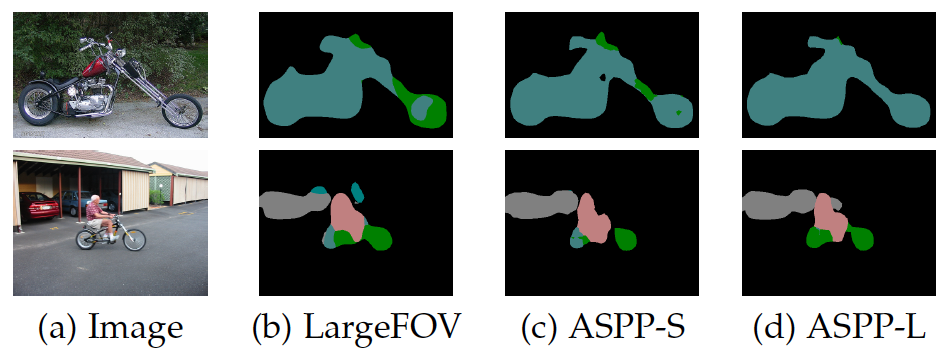
\includegraphics[width=0.7\textwidth]{figure/ss29.png}
	\captionsetup{justification=centering}
	\caption{Qualitative segmentation results of ASPP compared to the baseline LargeFOV model. {\color{blue}LargeFOV}: single branch, r = 12. {\color{blue}ASPP-S}: four branches, $r=\{2, 4, 8, 12\}$, {\color{blue}ASPP-L}: four branches, $r = \{6, 12, 18, 24\}$.}
\end{figure}
\end{frame}

\begin{frame}{Pascal VOC 2012: Qualitative Results}
\begin{itemize}
	\item Employing the {\color{blue}CRF} further improves the performance by removing false positives and refining object boundaries.
\end{itemize}	
\begin{figure}
	\centering
	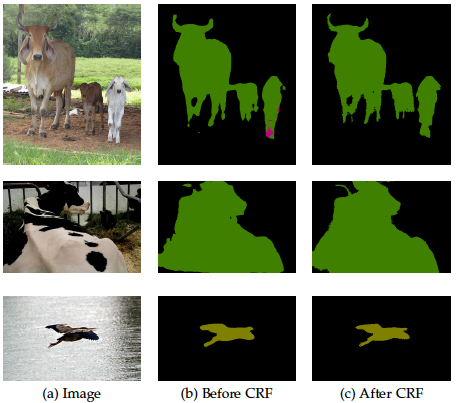
\includegraphics[width=0.40\textwidth]{figure/ss30.png}
	\captionsetup{justification=centering}
	\caption{Qualitative segmentation results before/after CRF.}
\end{figure}
\end{frame}

\begin{frame}{Pascal VOC 2012: Adopting Resnet-101}
\setbeamercovered{invisible}
\vspace{-0.2cm}
\begin{itemize}
	\item Adopting {\color{blue}ResNet-101} instead of VGG-16 significantly improves DeepLab performance.
\end{itemize}	
\vspace{-0.4cm}
\begin{table}
	\scalebox{0.8}{		
		\begin{tabular}{ c c c c c c | c }
			\hline{}
			\rule{0pt}{2.5ex}    
			MSC & COCO  & Aug & LFOV & ASPP & CRF & \textbf{mIOU} \\
			\hline
			& & & & & & $68.72$ \\
			\checkmark & & & & & & $71.27$ \\
			\checkmark & \checkmark & & & & & $73.28$ \\
			\checkmark & \checkmark & \checkmark & \checkmark & & & $74.87$ \\
			\checkmark & \checkmark & \checkmark & \checkmark & & & $75.54$ \\
			\checkmark & \checkmark & \checkmark & & \checkmark & & $76.35$ \\	
			{\color{green}\checkmark} & {\color{green}\checkmark} & {\color{green}\checkmark} & & {\color{green}\checkmark} & {\color{green}\checkmark} & {\color{green}$\vartriangleright$} {\color{green}$77.69$} {\color{green}$\vartriangleleft$} \\
		\hline		
		\end{tabular}
	}
	\captionsetup{justification=centering}
	\caption{Deeplab results on PASCAL VOC 2012 {\color{blue}VAL} set.\\ {\color{blue}MSC}: DCNN images at scale = $\{0.5, 0.75, 1\}$, {\color{blue}COCO}: MS-COCO dataset,\\ {\color{blue}Aug}: Randomly Scaled Input, {\color{blue}LFOV}: single branch,\\ {\color{blue}ASPP}: four branches, $r = \{6, 12, 18, 24\}$.}
\end{table}	
\end{frame}

\begin{frame}{Pascal VOC 2012: Qualitative Results}	
\begin{figure}
	\centering
	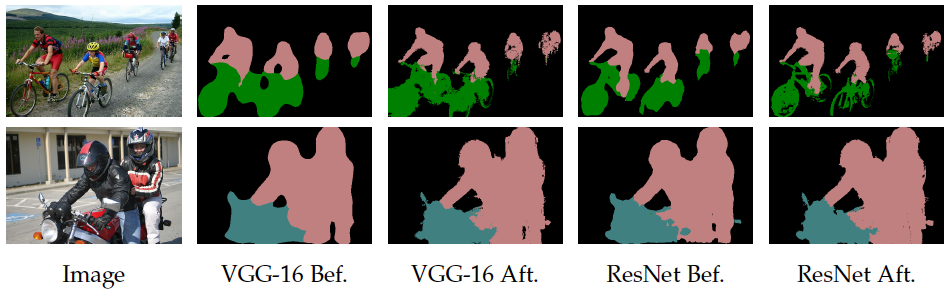
\includegraphics[width=0.70\textwidth]{figure/ss41.png}
	\captionsetup{justification=centering}
	\caption{DeepLab results.}
	\label{fig:M2}
\end{figure}
\vspace{-0.4cm}
\begin{itemize}
	\item Employing ResNet-101 without CRF has almost the same accuracy along object boundaries as employing VGG-16 with CRF procesing.
	\item Residual connections in ResNet-101 has similar effect as hyper-column features.
	%\item DeepLab results based on VGG-16 net or ResNet-101 before\\ and after CRF in {\color{blue}Figure \ref{fig:M2}}.
\end{itemize}
\end{frame}

\begin{frame}{Pascal VOC 2012: Qualitative Results}	
\begin{figure}
	\centering
	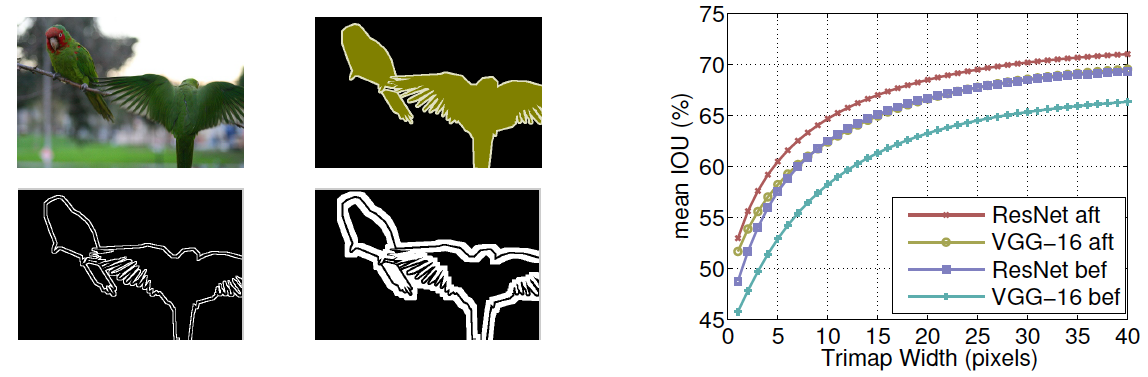
\includegraphics[width=0.70\textwidth]{figure/ss46.png}
	\captionsetup{justification=centering}
	\caption{Trimap examples(Left) and pixel IOU(right) as a function of trimap width.}
\end{figure}
\vspace{-0.4cm}
\begin{itemize}
	\item Using trimaps, one can evaluate segmentation accuracy around boundaries\footnote{Krähenbühl et al. "Efficient inference in fully connected CRFs with\\ gaussian edge potentials."}.
	\item Post-processing the ResNet-101 result with a CRF further improves the accuracy result.
\end{itemize}
\end{frame}

\begin{frame}{Pascal VOC 2012: Benchmark}	
	\begin{table}
		\scalebox{0.7}{
			\begin{tabular}{ l | c }
				\hline
				\textbf{Method} & \textbf{mIOU} \\
				\hline
				MERL\_DEEP\_GCRF & 73.2 \\
				CRF-RNN & 74.7 \\
				POSTECH\_DeconvNet\_CRF\_VOC & 74.8 \\
				BoxSup & 75.2 \\
				Context + CRF-RNN & 75.3 \\
				$\mathcal{Q}O_4^{mres}$ & 75.5 \\
				DeepLab-CRF-Attention & 75.7 \\
				CentraleSuperBoundaries++ & 76.0 \\
				DeepLab-CRF-Attention-DT & 76.3 \\
				H-ReNet + DenseCRF & 76.8 \\
				LRR\_4x\_COCO & 76.8 \\
				DPN & 77.5 \\
				Adelaide\_Context & 77.8 \\
				Oxford\textunderscore TVG\_HO\_CRF & 77.9 \\
				Context CRF + Guidance CRF & 78.1 \\
				{\color{red}Adelaide\_VeryDeep\_FCN\_VOC} & {\color{red}79.1} \\
				\hline 
				DeepLab-ASPP-L-CRF & 72.6 \\
				DeepLab-CRF-LargeFOV-COCO & 72.7 \\
				{\color{green}DeepLab-CRF (ResNet-101)} & {\color{green}$\vartriangleright$} {\color{green}$79.7$} {\color{green}$\vartriangleleft$} \\
				\hline 
			\end{tabular}
		}
		\captionsetup{justification=centering}
		\caption{Benchmark on PASCAL VOC 2012 {\color{blue}test} set.}
	\end{table}	
\end{frame}

\begin{frame}{PASCAL-Context: Dataset}	
\vspace{-0.3cm}
\begin{figure}
	\centering
	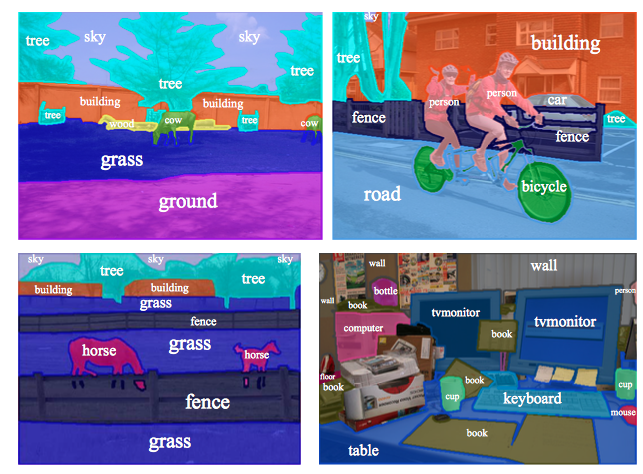
\includegraphics[width=0.50\textwidth]{figure/ss45.png}
	\captionsetup{justification=centering}
	\caption{Sample annotations.}
\end{figure}
\vspace{-0.5cm}
\begin{itemize}
	\item PASCAL-Context\footnote{Mottaghi, Roozbeh, et al. "The role of context for object detection\\ and semantic segmentation in the wild."} dataset provides semantic labels for the whole scene.
	\item Includes {\color{blue}4998} training, {\color{blue}5105} validation and {\color{blue}9637} test images.
	\item Out of {\color{blue}400+} classes, results are reported on the the most frequent {\color{blue}59}.
\end{itemize}
\end{frame}

\begin{frame}{PASCAL-Context: Evaluation}	
\vspace{-0.2cm}
\begin{table}
	\setlength{\tabcolsep}{3pt}
	\scalebox{0.8}{	
		\begin{tabular}{c c c c c c | c }
			\hline
			\rule{0pt}{2.5ex}    
			MSC & COCO & Aug & LargeFOV & ASPP & CRF & \textbf{mIOU} \\
			\hline
			\textit{VGG-16} & & & & & & \\
			& & & {\only<1>{\color{red}}\checkmark} & & & {\only<1>{\color{red}$\vartriangleright$}} {\only<1>{\color{red}}$37.6$} {\only<1>{\color{red}$\vartriangleleft$}} \\
			& & & {\only<2>{\color{red}}\checkmark} & & {\only<2>{\color{red}}\checkmark} & {\only<2>{\color{red}$\vartriangleright$}} {\only<2>{\color{red}}$39.6$} {\only<2>{\color{red}$\vartriangleleft$}} \\
			\hline
			\textit{ResNet-101} & & & & & & \\
			& & & & & & {\only<3>{\color{red}$\vartriangleright$}} {\only<3>{\color{red}}$39.6$} {\only<3>{\color{red}$\vartriangleleft$}} \\				
			{\only<4>{\color{red}}\checkmark} & & {\only<4>{\color{red}}\checkmark} & & & & {\only<4>{\color{red}$\vartriangleright$}} {\only<4>{\color{red}}$41.4$} {\only<4>{\color{red}$\vartriangleleft$}} \\
			{\only<5>{\color{red}}\checkmark} & {\only<5>{\color{red}}\checkmark} & {\only<5>{\color{red}}\checkmark} & & & & {\only<5>{\color{red}$\vartriangleright$}} {\only<5>{\color{red}}$42.9$} {\only<5>{\color{red}$\vartriangleleft$}} \\		
			{\only<6>{\color{red}}\checkmark} & {\only<6>{\color{red}}\checkmark} & {\only<6>{\color{red}}\checkmark} & {\only<6>{\color{red}}\checkmark} & & & {\only<6>{\color{red}$\vartriangleright$}} {\only<6>{\color{red}}$43.5$} {\only<6>{\color{red}$\vartriangleleft$}} \\		
			{\only<7>{\color{red}}\checkmark} & {\only<7>{\color{red}}\checkmark} & {\only<7>{\color{red}}\checkmark} & & {\only<7>{\color{red}}\checkmark} & & {\only<7>{\color{red}$\vartriangleright$}} {\only<7>{\color{red}}$44.7$} {\only<7>{\color{red}$\vartriangleleft$}} \\
			{\only<8>{\color{green}}\checkmark} & {\only<8>{\color{green}}\checkmark} & {\only<8>{\color{green}}\checkmark} & & {\only<8>{\color{green}}\checkmark} & {\only<8>{\color{green}}\checkmark} & {\only<8>{\color{green}$\vartriangleright$}} {\only<8>{\color{green}}$45.7$} {\only<8>{\color{green}$\vartriangleleft$}} \\		
			\hline					
		\end{tabular}
	}
	\captionsetup{justification=centering}
	\caption{Deeplab results on PASCAL Context {\color{blue}test} set. {\color{blue}MSC}: DCNN images at scale = $\{0.5, 0.75, 1\}$, {\color{blue}COCO}: MS-COCO dataset,  {\color{blue}Aug}: Randomly Scaled Input, {\color{blue}LargeFOV}: single branch, {\color{blue}ASPP}: four branches, $r = \{6, 12, 18, 24\}$.}		
\end{table}
\end{frame}

\begin{frame}{Pascal-Context: Benchmark}	
\vspace{-0.3cm}
\begin{itemize}
	\item Final model yields {\color{blue}$45.7\%$}, outperforming the current state-of-art method.
\end{itemize}
\vspace{-0.5cm}
\begin{table}
	\scalebox{0.8}{
		\begin{tabular}{ l | c }
			\hline
			\textbf{Method} & \textbf{mIOU} \\
			\hline
			O2P & 18.1 \\
			CFM & 34.4 \\
			FCN-8s & 37.8 \\
			CRF-RNN & 39.3 \\
			ParseNet & 40.4 \\
			BoxSup & 40.5 \\
			HO\_CRF & 41.3 \\
			Context & 43.3 \\
			VeryDeep & {\color{red}44.5} \\
			\hline 
			DeepLab-MSC-COCO-Aug-ASPP-&\\
			CRF (VGG-16) & {\color{green}$\vartriangleright$} {\color{green}$45.7$} {\color{green}$\vartriangleleft$} \\
			\hline 
		\end{tabular}
	}
	\captionsetup{justification=centering}
	\caption{Benchmark results on PASCAL Context test set. {\color{blue}MSC}: DCNN images at scale = $\{0.5, 0.75, 1\}$, {\color{blue}COCO}: MS-COCO dataset,  {\color{blue}Aug}: Randomly Scaled Input, {\color{blue}ASPP}: four branches, $r = \{6, 12, 18, 24\}$.}		
\end{table}	
\end{frame}

\begin{frame}{PASCAL-Context: Qualitative Results}	
\begin{itemize}
	\item CRF helps improve the model by removing false positives and improving the prediction along object boundaries({\color{blue}Figure \ref{fig:M3}}).
\end{itemize}

\begin{figure}
	\centering
	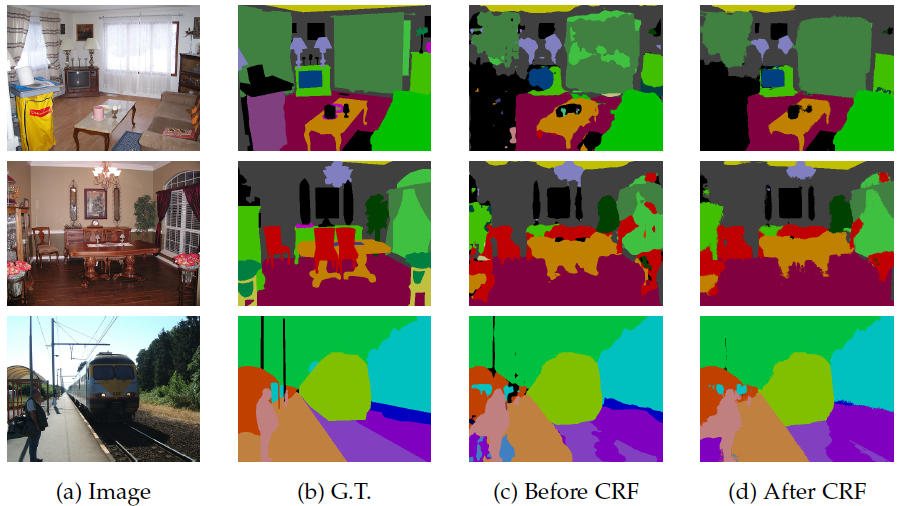
\includegraphics[width=0.60\textwidth]{figure/ss32.png}
	\captionsetup{justification=centering}
	\caption{PASCAL-Context results.}
	\label{fig:M3}
\end{figure}
\vspace{-0.4cm}
\end{frame}

\begin{frame}{PASCAL-Person-Part: Dataset}
\vspace{-0.4cm}
\begin{figure}
	\centering
	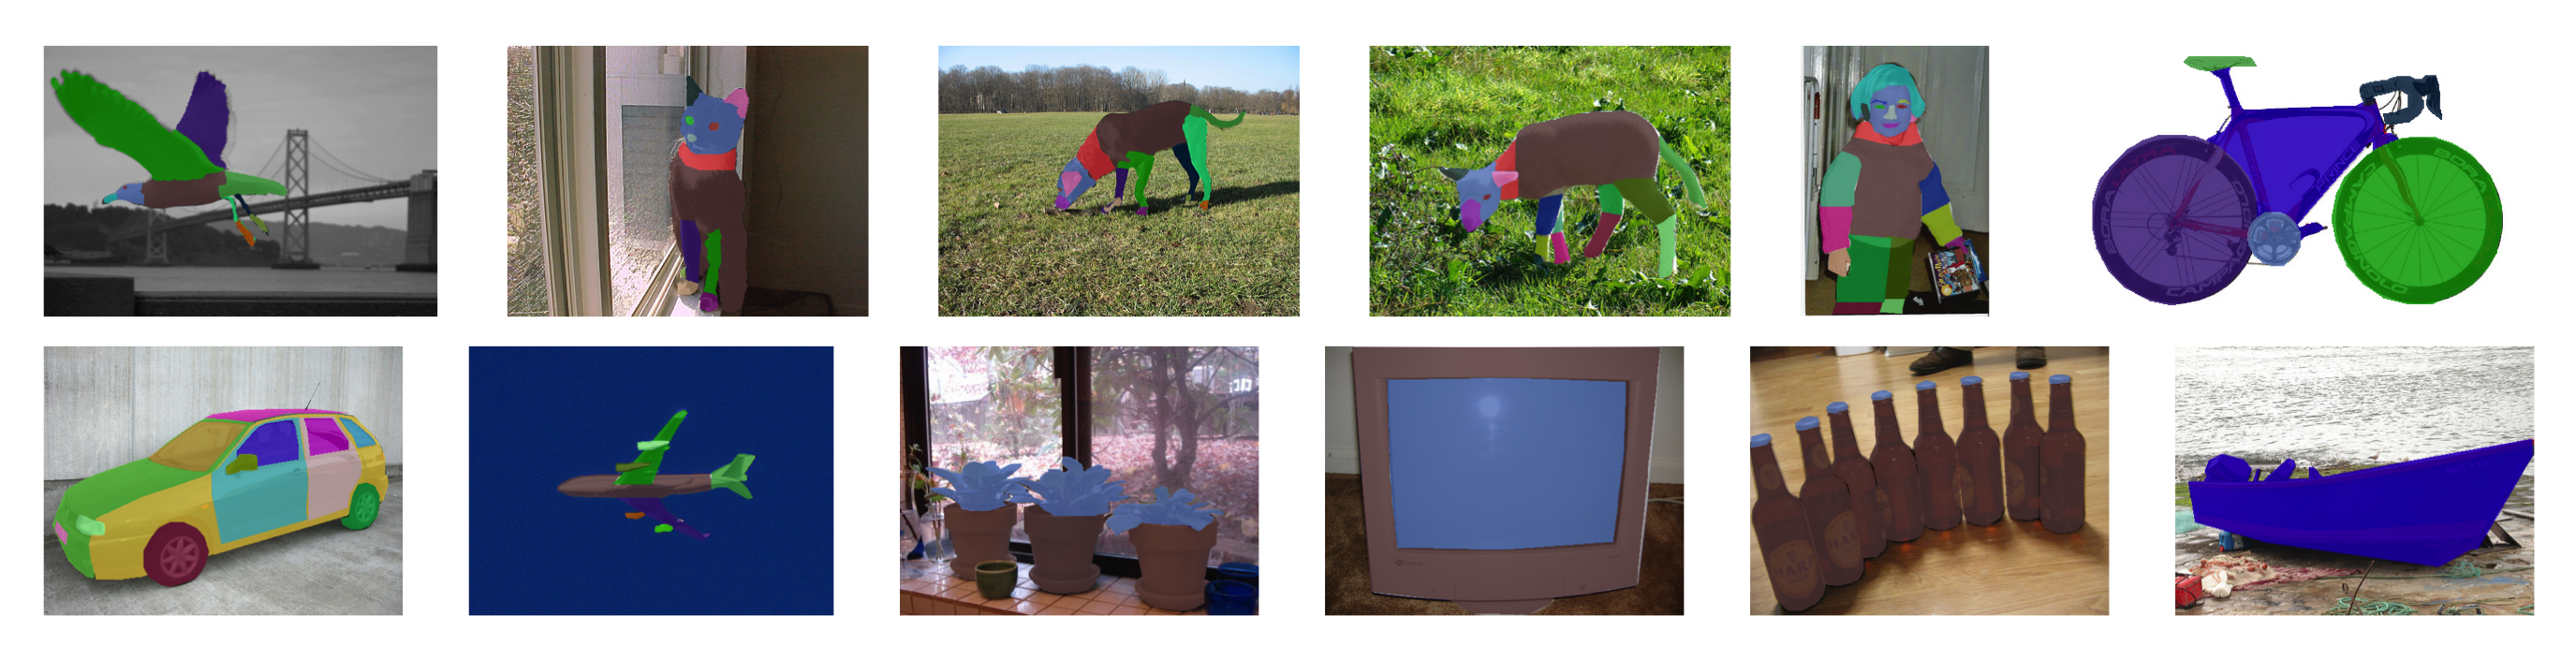
\includegraphics[width=0.7\textwidth]{figure/ss33.png}
	\captionsetup{justification=centering}
	\caption{PASCAL-Part-Dataset\footnote{http://www.stat.ucla.edu/pascal\_part\_dataset/pascal\_part.html}.}
\end{figure}
\vspace{-0.6cm}
\begin{itemize}
	\item {\color{blue}PASCAL-Part-Dataset}\footnote{Chen, Xianjie, et al. "Detect what you can: Detecting and representing\\ objects using holistic models and body parts. (2014)"} provides segmentation masks for each body part of the object.
	\item The dataset contains detailed part annotations for every person \textit{e.g.} eyes, nose etc.
	\item Annotations are merged to be \emph{Head, Torso, Upper/Lower Arms and Upper/Lower Legs}.
\end{itemize}	
\end{frame}

\begin{frame}{PASCAL-Person-Part: Evaluation}
\begin{table}
	\scalebox{0.8}{	
		\begin{tabular}{l c c c c c c | c }
			\hline{}
			\rule{0pt}{2.5ex}    
			Method & MSC & COCO  & Aug & LFOV & ASPP & CRF & \textbf{mIOU} \\
			\hline
			\textit{ResNet-101} & & & & & & & \\
			DeepLab & & & & & & & $58.90$ \\
			DeepLab & \checkmark & & \checkmark & & & & $63.10$ \\
			DeepLab & \checkmark & \checkmark & \checkmark & & & & $64.40$  \\
			{\color{green}DeepLab} & {\color{green}\checkmark} & {\color{green}\checkmark} & {\color{green}\checkmark} & & &{\color{green}\checkmark} & {\color{green}$\vartriangleright$} {\color{green}$64.94$} {\color{green}$\vartriangleleft$} \\		
			\hline
			\textit{VGG-16} & & & & & & & \\
			DeepLab & \checkmark & \checkmark & \checkmark & \checkmark & & & $62.18$ \\
			DeepLab & \checkmark & \checkmark & \checkmark & & \checkmark & & $62.76$ \\												
			\hline
			\hline
			Attention & & & & & & & 56.39 \\
			HAZN & & & & & & & 57.54 \\
			LG-LSTM & & & & & & & 57.97 \\
			{\color{red}Graph LSTM} & & & & & & & {\color{red}60.16} \\
			\hline			
		\end{tabular}
	}
   	\captionsetup{justification=centering}
	\caption{DeepLab results on PASCAL-Person-Part {\color{blue}VAL} set.\\{\color{blue}MSC}: DCNN images at scale = $\{0.5, 0.75, 1\}$, {\color{blue}COCO}: MS-COCO dataset,  \\{\color{blue}Aug}: Randomly Scaled Input, {\color{blue}LargeFOV}: single branch,\\{\color{blue}ASPP}: four branches, $r = \{6, 12, 18, 24\}$.}
\end{table}	
\end{frame}

\begin{frame}{PASCAL-Person-Part: Qualitative Results}	
\begin{itemize}
	\item Dense CRF is used to post process final output, advancing the state-of-the-art on the PASCAL-Person-Part dataset.
\end{itemize}	
\begin{figure}
	\centering
	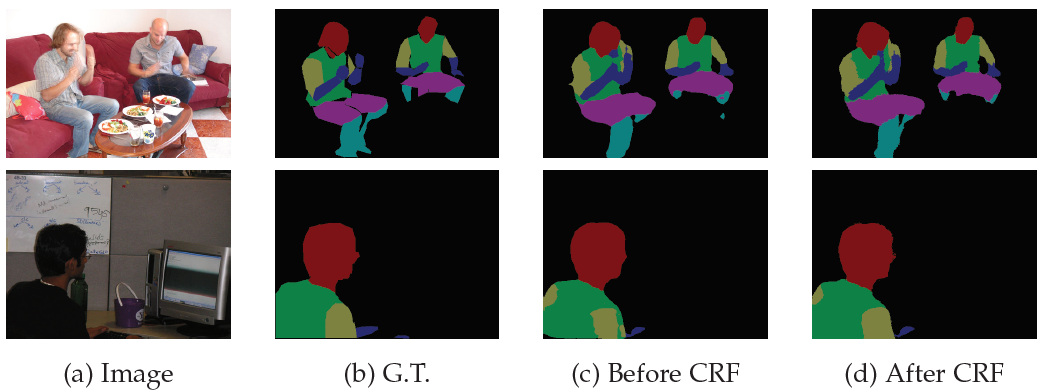
\includegraphics[width=0.80\textwidth]{figure/ss48.png}
	\captionsetup{justification=centering}
	\caption{Qualitative results on PASCAL-Person-Part dataset.}
	\label{fig:M4}
\end{figure}
\end{frame}

\begin{frame}{Cityscapes: Dataset}	
\begin{figure}
	\centering
	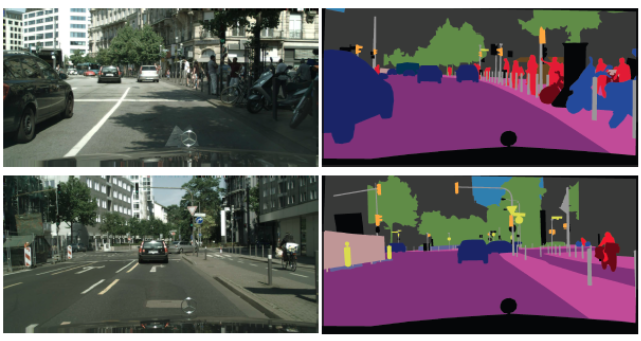
\includegraphics[width=0.50\textwidth]{figure/ss38.png}
	\captionsetup{justification=centering}
	\caption{Cityscapes dataset\footnotemark[\getrefnumber{label3}].}
\end{figure}
\vspace{-0.5cm}
\begin{itemize}
	\item {\color{blue}5000} images collected in street scenes from {\color{blue}50} different cities\footnote{MLA	
		Cordts, Marius, et al. "The cityscapes dataset for semantic urban\\ scene understanding. (2016)" \label{label3}}.
	\item {\color{blue}2975}, {\color{blue}500}, and {\color{blue}1525} training, validation, and test images\\ respectively.
	\item Out of {\color{blue}30}, {\color{blue}19} most frequent semantic labels (belonging to {\color{blue}7 super categories}: ground, construction, object, nature, sky, human, and vehicle) are used for evaluation.
\end{itemize}
\end{frame}

\begin{frame}{Cityscapes: Evaluation}	
\begin{itemize}
\item Model trained with subsampled images or each image is split into overlapped regions({\color{blue}full}).
\end{itemize}
\vspace{-0.2cm}
\begin{table}
	\setlength{\tabcolsep}{3pt}
	\scalebox{0.8}{	
		\begin{tabular}{ c c c c c | c }
			\hline
			\rule{0pt}{2.5ex}    
			Full & Aug & LargeFOV  & ASPP & CRF & \textbf{mIOU} \\
			\hline
			\textit{VGG-16} & & & & & \\
		 	& & \checkmark & & & $62.97$ \\
		 	& & \checkmark & & \checkmark & $64.18$	 \\
		 	\checkmark & & \checkmark & & & $64.89$ \\	 	
		 	\checkmark & & \checkmark & & \checkmark & $65.94$ \\	 	
		 	\hline 
			\textit{Resnet-101} & & & & & \\	 	
			\checkmark & & & & & $66.6$ \\
			\checkmark & & \checkmark & & & $69.2$ \\
			\checkmark & & & \checkmark & & $70.4$ \\
			\checkmark & \checkmark & & \checkmark & & $71.0$ \\
			{\color{green}\checkmark} & {\color{green}\checkmark} & & {\color{green}\checkmark} & {\color{green}\checkmark} &  {\color{green}$71.4$} \\	
			\hline					
		\end{tabular}
	}
   	\captionsetup{justification=centering}
	\caption{DeepLab results on Cityscapes validation set.\\{\color{blue}Full}: Model trained with full resolution images($2048\times1024$). {\color{blue}Aug}:\\ Randomly Scaled Input, {\color{blue}LargeFOV}: single branch, {\color{blue}ASPP}:\\ four branches, $r = \{6, 12, 18, 24\}$.}
\end{table}
\end{frame}

\begin{frame}{Cityscapes: Benchmark}	
\vspace{-0.4cm}
\begin{table}
	\captionsetup{justification=centering}
	\caption{Benchmark results on PASCAL Context test set. {\color{blue}MSC}: DCNN images at scale = $\{0.5, 0.75, 1\}$, {\color{blue}COCO}: MS-COCO dataset, {\color{blue}Aug}: Randomly Scaled Input, {\color{blue}ASPP}: four branches, $r = \{6, 12, 18, 24\}$.}	
	\scalebox{0.8}{
		\begin{tabular}{ l | c }
			\hline
			\textbf{Method} & \textbf{mIOU} \\
			\hline
			\textit{pre-release version of dataset} & \\
			Adelaide\_Context & 66.4 \\
			FCN-8s & 65.3 \\
			\hline
			DeepLab-CRF-LargeFOV-StrongWeak & 64.8 \\
			DeepLab-CRF-LargeFOV & 63.1 \\
			\hline
			CRF-RNN & 62.5 \\
			DPN & 59.1 \\
			Segnet basic & 57.0 \\
			Segnet extended & 56.1 \\
			\hline
			\hline
			\textit{official version} & \\
			Adelaide\_Context & 71.6 \\
			Dilation10 & 67.1 \\
			DPN & 66.8 \\
			Pixel-level Encoding & 64.3 \\
			\hline
			{\color{green}DeepLab-CRF (ResNet-101)} & {\color{green}70.4} \\
			\hline
		\end{tabular}
	}	
\end{table}	
\end{frame}



\begin{frame}{Cityscapes: Qualitative Results}	
\begin{figure}
	\centering
	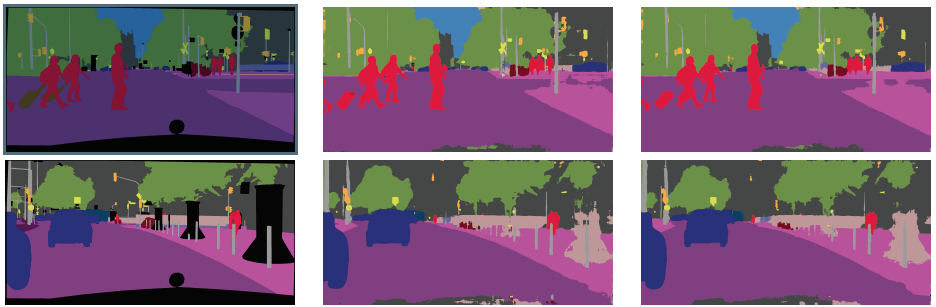
\includegraphics[width=0.90\textwidth]{figure/ss39.png}
	\captionsetup{justification=centering}
	\caption{Qualitative results on Cityscapes dataset.}
	\label{fig:M6}
\end{figure}
\end{frame}

\begin{frame}{Failure Modes}	
	\begin{figure}
		\centering
		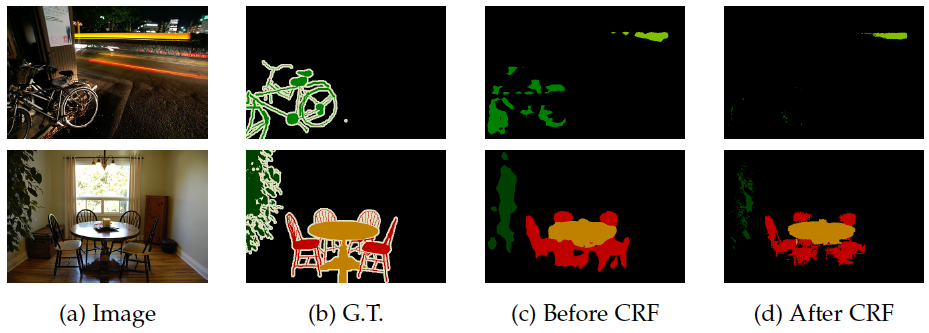
\includegraphics[width=0.90\textwidth]{figure/ss49.png}
		\captionsetup{justification=centering}
		\caption{Failure modes.}
		\label{fig:M10}
		\vspace{-0.4cm}
		\begin{itemize}
		\item Deeplab fails to capture the delicate boundaries of objects, such as bicycle and chair as shown in Fig. \ref{fig:M10}.
		\item CRF post processing fails since the \emph{unary term} is not confident enough.
		\end{itemize}
	\end{figure}
\end{frame}

\setbeamercovered{transparent}
\section{Future Direction}
\begin{frame}{Future Direction}
\begin{itemize}
\item<1-> {\color{blue}Weaker supervision\footnote{Papandreou, George, et al. "Weakly-and semi-supervised learning of\\ a DCNN for semantic image segmentation. (2015)" }} has been conducted in a number of papers, not requiring that pixel-level semantic annotations are available for the whole training set.
\item<2-> {\color{blue}End-to-end CRF+DCNN} learning methods could be investigated.
\item<3-> DeepLab can be applied on other {\color{blue}end-to-end regression tasks}, i.e depth/optical flow prediction, super-resolution estimation, denoising, demosaicing, bottom-up saliency, keypoint detection etc.
\item<4-> To capture delicate boundaries, {\color{blue}fine-grained features} can be incorporated.
\end{itemize}
\end{frame}

\section{Appendix}
\setbeamercovered{invisible}
\begin{frame}{Appendix: Mean Field Approximation}
\begin{itemize}
	\item Key idea\footnote{Krähenbühl et al. "Efficient inference in fully connected CRFs with\\ gaussian edge potentials."}: Instead of computing the exact distribution, find a distribution $\mathcal{Q}(\mathbf{X})$ that minimizes the KL-divergence $\mathbf{D}(\mathcal{Q}\lVert P)$.
	\item Distribution $\mathcal{Q}$ can be expressed as a product of independent marginals, $\mathcal{Q}(\mathbf{X})=\prod_i{\mathcal{Q}_i(\mathbf{X_i})}$ 
\end{itemize}
\vspace{-0.6cm}
\begin{table}
\begin{tabular}{@{}l l@{}}
		\hline
		\rule{0pt}{2.5ex}    				
		\textbf{Algorithm 1} Mean field for FC-CRF &   \\
		\hline 
		\rule{0pt}{2.5ex}    		
		\hspace{-0.17cm}Initialize $\mathcal{Q}$  &  $\vartriangleright \mathcal{Q}_i(x_i) \leftarrow \frac{1}{Z_i}\exp\{-\theta_i(x_i)\} $ \\
		\textbf{while} not converged \textbf{do} \onslide<2-> &\\ 
		\hspace{0.2cm}$\tilde{\mathcal{Q}}_i^{(m)}(l)\leftarrow\sum_{j\neq i}k^{(m)}( \mathbf{f_i,f_j} )\mathcal{Q}_j(l) \text{ for all } m$ & $\vartriangleright$ \textbf{MP} from all $X_j$ to all $X_i$ \onslide<3->\\ 
		\hspace{0.2cm}$\hat{\mathcal{Q}}_i(x_i)  \leftarrow \sum_{l\in\mathcal{L}}\mu^{(m)}(x_i,l)\sum_m 	w^{(m)}\tilde{\mathcal{Q}}_i^{(m)} $ &  $\vartriangleright$ \textbf{Compatibility transform } \onslide<4->\\
		\hspace{0.2cm}$\mathcal{Q}_i(x_i)  \leftarrow \exp\{-\theta_i(x_i)- \hat{\mathcal{Q}}_i(x_i) \} $  & $\vartriangleright$ \textbf{Local Update } \onslide<5->\\
		\hspace{0.2cm}Normalize $\mathcal{Q}_i(x_i) $ & \\
		\textbf{end while} 
	\end{tabular}
\end{table}
\end{frame}

\begin{frame}{Appendix: Mean Field Approximation}
\begin{itemize}
	\item Qualitative results:
\end{itemize}
\begin{figure}
	\centering
	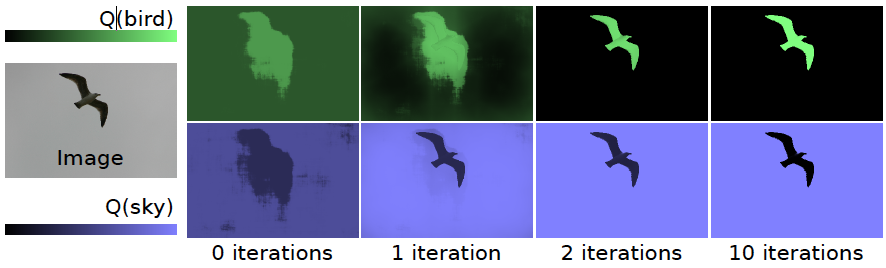
\includegraphics[width=0.80\textwidth]{figure/ss50.png}
	\captionsetup{justification=centering}
	\caption{Distributions $\mathcal{Q}(X_i=\text{\enquote*{bird}) (top)} \text{ and } \mathcal{Q}(X_i=\text{\enquote*{sky})}$ (bottom)}.
	\label{fig:M11}
\end{figure}

\end{frame}

\begin{frame}{Appendix: Mean Field Approximation}
\begin{itemize}
	\item \textit{Compatibility transform} and the \textit{local update} run in linear time.
	\item MP step can be expressed as a convolution with a Gaussian kernel in feature space.
	\item By the sampling theorem\footnote{S. W. Smith. The scientist and engineer’s guide to digital signal processing.}, function ${\mathcal{Q}(l)}$ can be reconstructed from a set of samples whose spacing is proportional to the standard deviation of the filter.
	\item Use truncated Gaussian, where all values beyond two standard deviations are set to zero.
	\item Perform the convolution by downsampling.
	\item Convolution computed at each sample uses values from a constant number of neighbour samples.
	\item This implies that approx. MP can be performed in $O(N)$.
\end{itemize}
\end{frame}

\end{document}
